\chapter{Étude de cas - défaillance circuit intégré}
\label{chap:3}
\section{Présentation du produit et de la défaillance}

Ce travail de recherche a pour but d'étudier et de prédire les pertes de fonctionnalités causées par des décharges électrostatiques.
Dans ce chapitre, un cas réel de défaillance fonctionnelle est présenté.
Il a été identifié sur un circuit intégré automobile spécifique, qui a pour responsabilité des tâches critiques et de haut-niveau dans le véhicule.
Cette défaillance a été détectée en réduisant la quantité de composants externes au niveau de la carte, dans le but de diminuer la BOM (Bill Of Materials) et donc le coût de l'application complète.
Dans la campagne de tests, les décharges sont injectées à travers la connexion batterie (Fig. \ref{fig:system_architecture}).

\begin{figure}[!h]
  \centering
  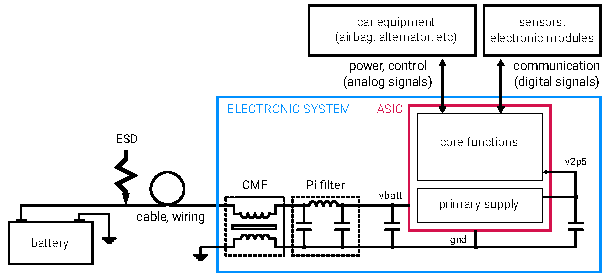
\includegraphics[width=0.9\textwidth]{src/1/figures/architecture_system.pdf}
  \caption{Vue d'ensemble de l'architecture du système}
  \label{fig:system_architecture}
\end{figure}

% Main task
La tâche en défaillance est une fonction de régulation, chargée principalement de convertir la tension batterie en une alimentation régulée 2.5 V.
Plusieurs sous-fonctions (aussi appelées blocs) traitent la tension batterie dans ce but.
L'architecture de la fonction intégrée est donnée Fig. \ref{fig:monitored_function}).

\begin{figure}[!h]
  \centering
  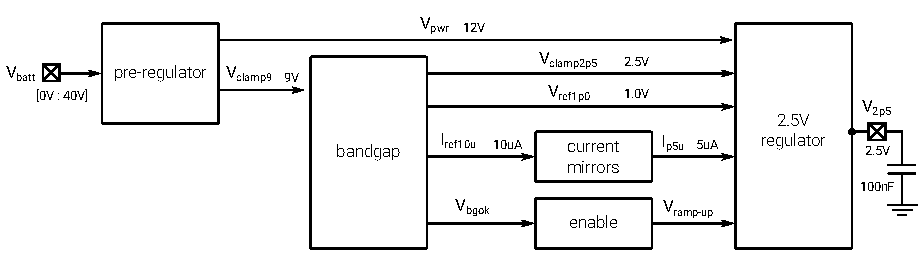
\includegraphics[width=0.9\textwidth]{src/1/figures/monitored_function.pdf}
  \caption{Architecture du primaire d'alimentation}
  \label{fig:monitored_function}
\end{figure}

% First block
Le pré-régulateur limite la tension d'entrée V\textsubscript{batt} pouvant atteindre jusqu'à 40 V, et fournit le signal V\textsubscript{clamp9}.
V\textsubscript{clamp9} alimente les blocs internes à faible consommation, tandis que V\textsubscript{pwr} fournit un plus large courant sous 12 V.
% Second block
Ensuite, une référence bandgap génère, après un délai de démarrage, notamment une référence à 1.0 V appelée V\textsubscript{ref1p0}.
Le bandgap fournit aussi une référence de courant à 10\textMu{}A sur I\textsubscript{ref10u}, ainsi qu'un drapeau V\textsubscript{bgok} pour signaler si il est en fonctionnement nominal ou non .
% Third major block
Enfin, le régulateur faible-pertes génère une alimentation stabilisée 2.5 V sur V\textsubscript{2p5}, avec une capacité en courant jusqu'à 20 mA.
V\textsubscript{2p5} sert ensuite à alimenter des cellules digitales à l'intérieur du circuit intégré.

% Principe défaillance
La défaillance de ce système est observée sur V\textsubscript{2p5} (Fig. \ref{fig:meas-reset-v2p5}).
Elle est induite en injectant une forte impulsion transitoire d'amplitude négative sur V\textsubscript{batt}, lorsque le produit est alimenté et en fonctionnement normal.
La durée de la défaillance sur V\textsubscript{2p5} (30 \textmu{}s) est bien plus longue que la perturbation d'entrée sur V\textsubscript{batt} (100 ns), ce qui semble indiquer une large faute fonctionnelle dans le circuit.

\begin{figure}[!h]
  \centering
  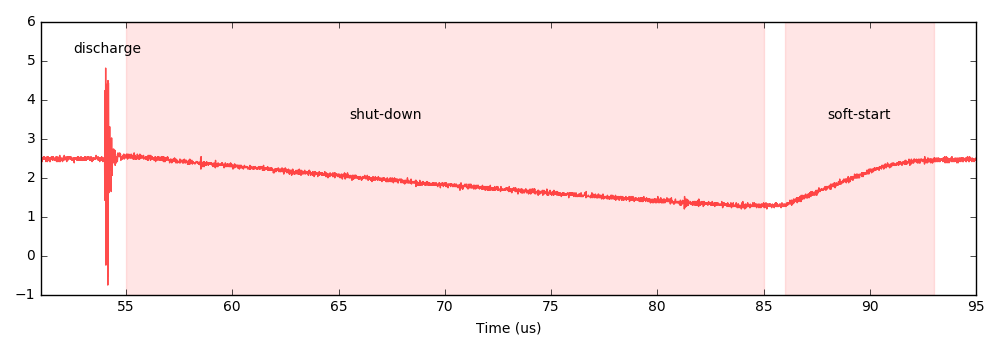
\includegraphics[width=0.9\textwidth]{src/1/figures/v2p5_measure.png}
  \caption{Mesure de V\textsubscript{2p5} après une stress rectangulaire -450 V 100 ns}
  \label{fig:meas-reset-v2p5}
\end{figure}

% What is the root cause -> reset of regulator, soft-start
Plus précisément, le stress négatif semble déclencher une séquence de démarrage, alors que le régulateur est normalement déjà démarré.
Pendant cette séquence, la tension d'alimentation monte doucement depuis 0 V jusqu'à 2.5 V, afin d'éviter des surtensions.
Ces séquences de démarrage sont logiquement longues et demandent un certain temps pour se terminer.
Si un ESD déclenche une telle séquence, le système se retrouve indisponible pendant un délai important.

La prochaine partie du travail de recherche est focalisé sur le développement de méthodes de mesures directement sur silicium.
L'objectif est d'acquérir des données fiables directement au niveau circuit, ce qui est difficile à faire de manière externe, et afin de valider les simulations pour l'investigation.
Notamment, un véhicule de test a été développé.
Il contient différentes méthodes de mesure et d'observation.

\section{Présentation du véhicule de test}

% Architecture
L'architecture du véhicule de test est donnée Fig. \ref{architecture_testchip}.
Il contient deux instances de la même fonction de régulation.
La première instance est la fonction sous-test, exposée à des décharges électrostatiques pendant la campagne de tests et dont le comportement est surveillé afin de détecter les fautes.
La seconde instance alimente justement les systèmes de surveillance qui sont directement intégrés sur puce.

\begin{figure}[h]
  \centering
  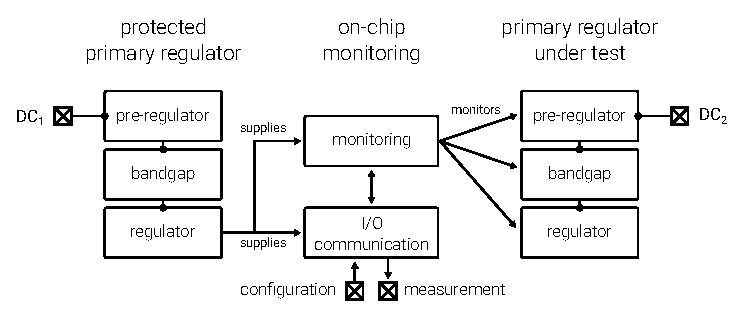
\includegraphics{src/1/figures/architecture_testchip.pdf}
  \caption{Architecture du véhicule de test}
  \label{architecture_testchip}
\end{figure}

Le layout top de la puce est donné Fig. \ref{fig:top-cell-layout}.
Il est possible d'identifier à droite et à gauche chaque instance de la fonction de régulation.
Les systèmes de surveillance sont localisés globalement de dessous de ces deux blocs.
Des capteurs de courant sur puce sont localisés à plusieurs endroit contre l'anneau de métal gndsub entourant toute la puce.
Beaucoup d'espace a été laissé libre sur le layout, pour des contraintes de fabrication.

\begin{figure}[!h]
  \centering
  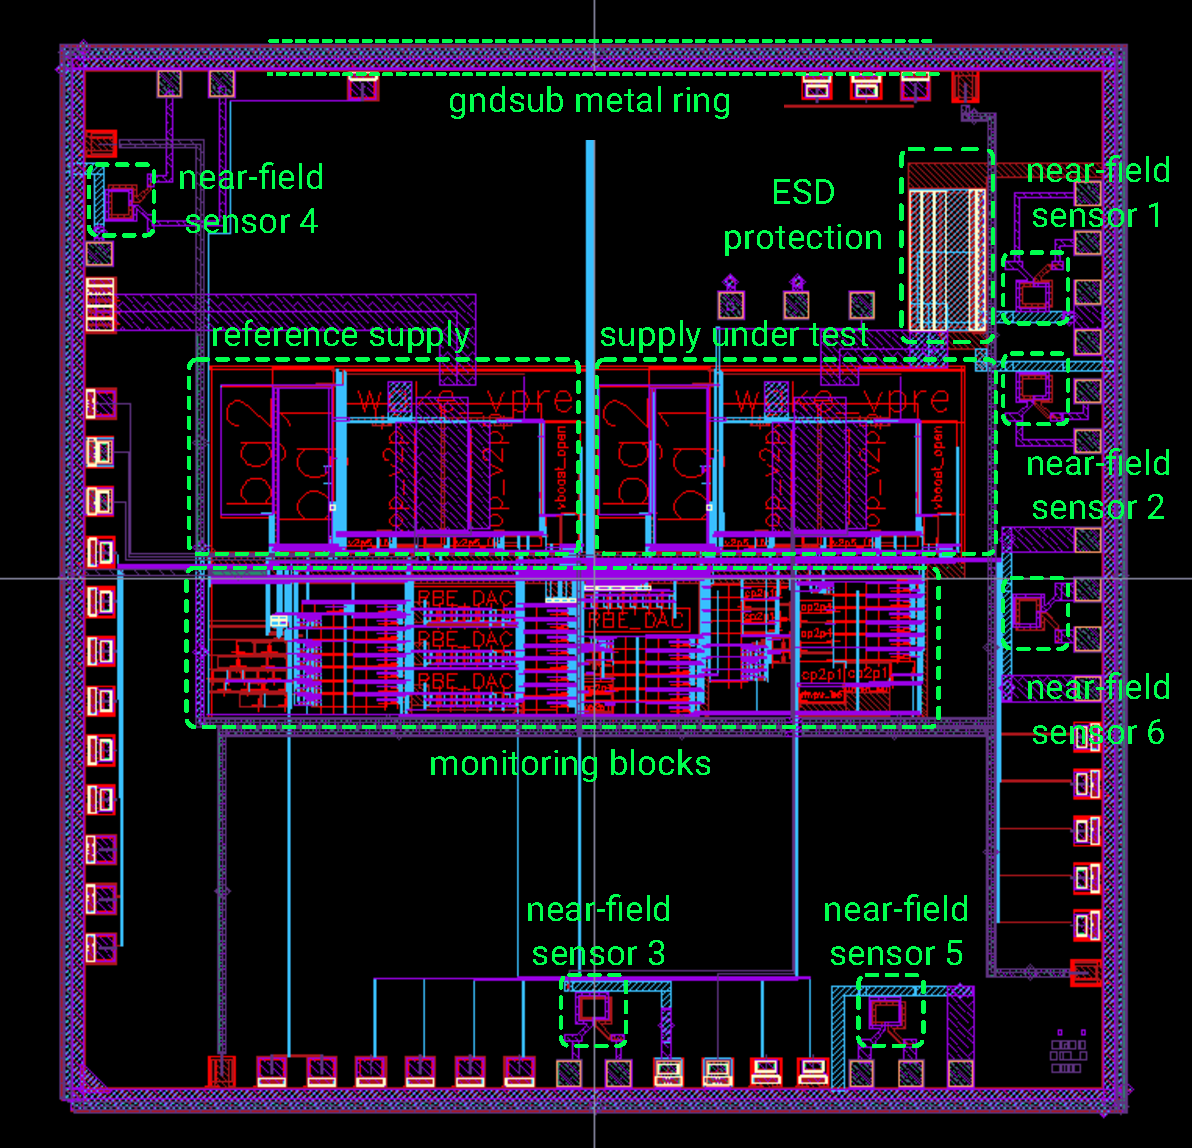
\includegraphics[width=0.7\textwidth]{src/1/figures/topcell_layout.pdf}
  \caption{Layout de la top-cell}
  \label{fig:top-cell-layout}
\end{figure}

% What is in the monitoring system
Les systèmes de surveillance contiennent notamment des détecteurs de surtension et sous-tension.
Il y a au total 35 détecteurs de ce type dans la puce.
Ils sont implémentés avec des comparateurs verrouillés
Un drapeau est levé si un nœud surveillé dépasse un niveau de référence.
Une fois le drapeau levé, il est maintenu jusqu'à ce que la cellule puisse être lue et remise � z�ro.
L'architecture est donnée Fig. \ref{fig:architecture-ov}.

\begin{figure}[!h]
  \centering
  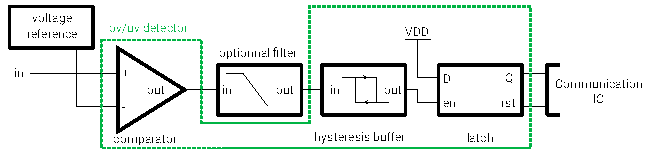
\includegraphics[width=0.9\textwidth]{src/1/figures/architecture_OV.pdf}
  \caption{Architecture du détecteur de surtension}
  \label{fig:architecture-ov}
\end{figure}

% Detail architecture
Dans cette architecture, la comparaison est réalisée par le comparateur, implémenté avec un amplificateur opérationnel à deux étages avec un buffer de sortie.
Cette topologie convient bien pour des comparateurs à fort gain, travaillant en boucle ouverte avec une très forte impédance d'entrée, afin de ne pas perturber le circuit.
A la sortie du comparateur, un filtre RC optionnel peut être connecté.
Il permet d'éliminer les surtensions les plus courtes afin de détecter seulement de larges perturbations.
Ensuite, un buffer à hystérésis permet de maximiser l'efficacité du filtre et d'obtenir une valeur numérique robuste de la sortie du comparateur.
Finalement, une bascule D garde le drapeau en mémoire une fois levé.
Si le buffer à hystérésis devient haut, la bascule recopie un état haut sur sa sortie.

% Origin of reference voltages
Les tensions de références de ces détecteurs sont soit fixes, soit contrôlables via un bus de communication.
Par ailleurs, tout ces détecteurs peuvent être lus par un second bus de communication.
Ce bus fonctionne sur le principe d'une chaine JTAG.
Des cellules individuelles peuvent être connectées en chaine afin de former un bus de la longueur désiré.
Cette approche est très pratique pour monter rapidement un véhicule de test.
Néanmoins, des problèmes important furent rencontrés avec ces bus de communication.
Ils sont exposés en détail dans le document complet.

% What is a current sensors
Dans le véhicule de test, on trouve également des capteurs de courant directement intégrés sur silicium.
Chaque capteur est placé à proximité de la piste de métal à mesurer.
Par couplage, il génère une tension proportionnelle à la dérivée du courant dans la piste.

La figure \ref{fig:near-field-current-sensor} donne une représentation 3D du capteur.
Ce type de boucle de courant intégré sur silicium a été originellement désigné et étudié par A. Salles dans \cite{AlainSallesInductors}.

\begin{figure}[!h]
  \centering
  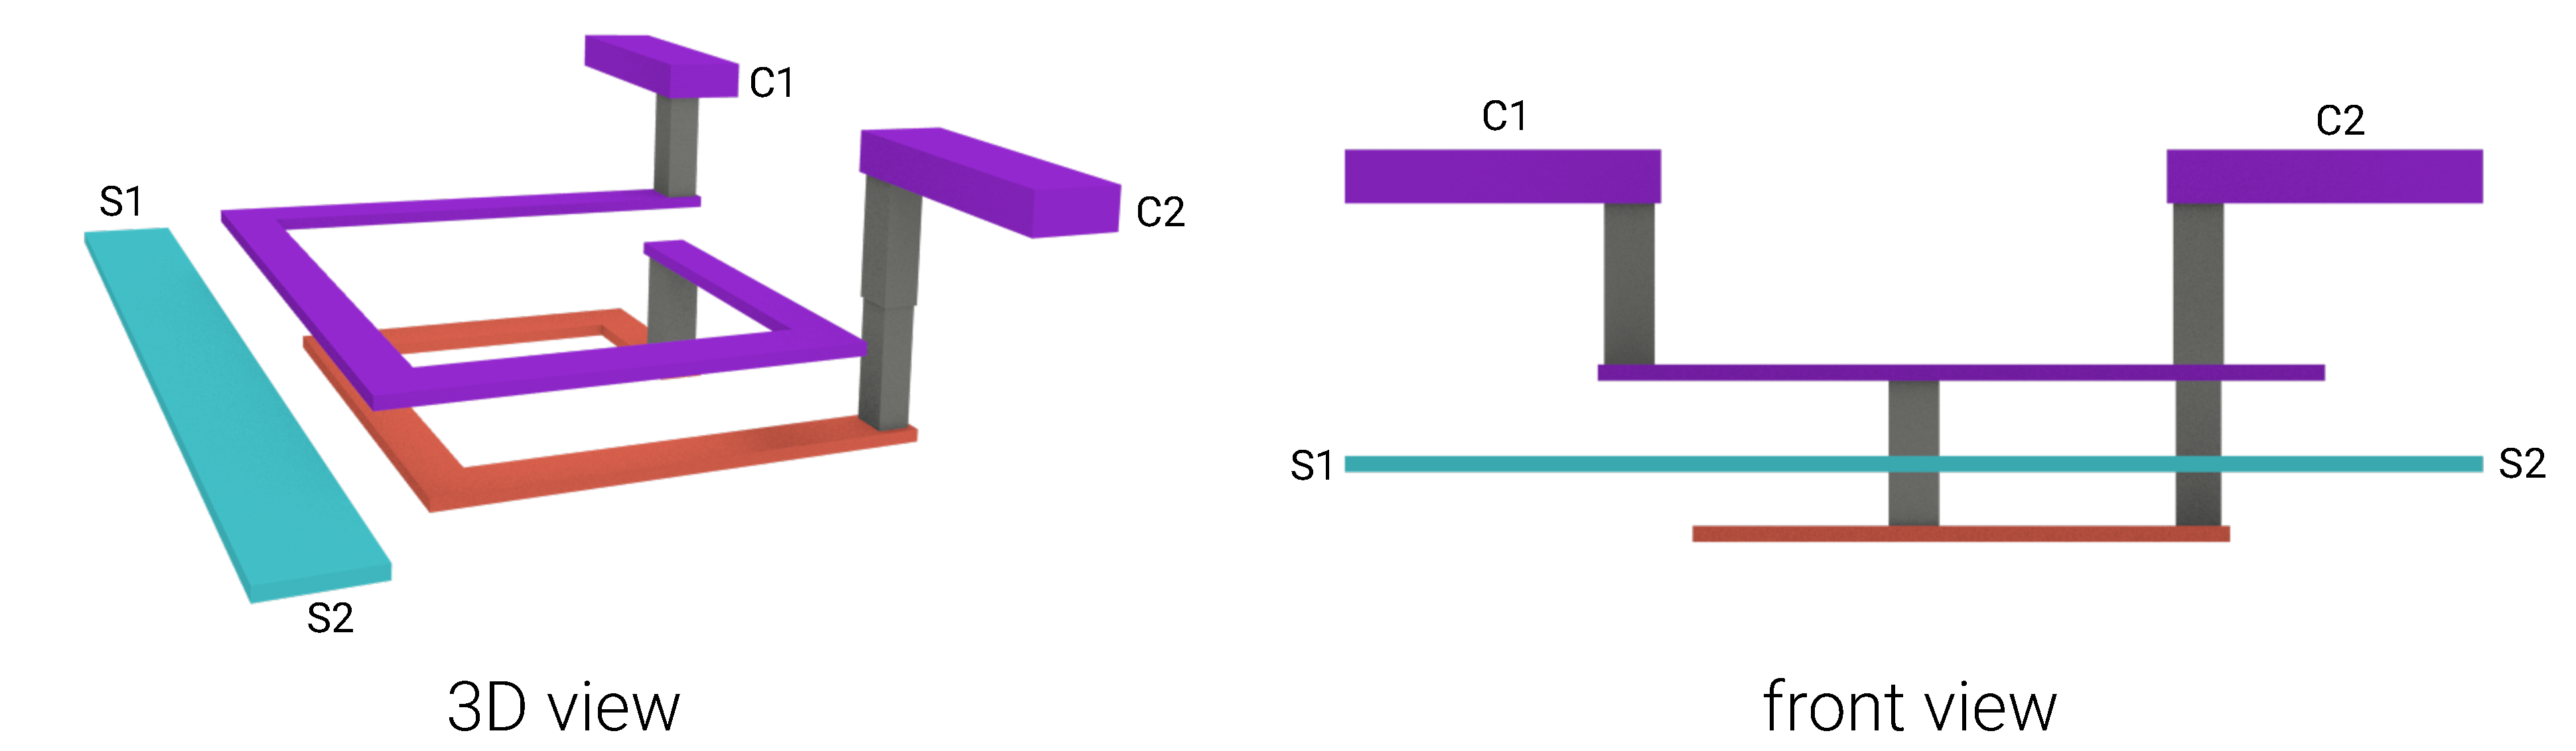
\includegraphics[width=0.98\textwidth]{src/1/figures/near-field-current-sensor.pdf}
  \caption{Design du capteur de champ-proche}
  \label{fig:near-field-current-sensor}
\end{figure}

% How is it designed and how is it used
Sur silicium, trois niveaux de métaux sont requis pour construire ce capteur.
Le premier niveau en rouge (Fig \ref{fig:near-field-current-sensor}) et le troisième niveau en violet forment une boucle métallique.
Des vias connectent les différents niveaux ensembles.
La piste mesurée est elle localisée au deuxième niveau.
Le courant mesuré circule entre les nœuds \textit{S1} et \textit{S2}.
Un oscilloscope avec une impédance d'entrée \textOmega{} est utilisé pour mesurer en différentiel la tension entre \textit{C1} et \textit{C2}.
Le traitement de la courbe obtenue a été détaillé précédemment dans le chapitre 2.

% Talk about the near-field current sensors placement
Au total, il y a 6 capteurs de courant sur la puce.
Un des capteurs est dédié à la calibration, tandis que les autres mesurent des points d'entrée ou de sortie potentiels pour des ESD.
Le capteur \textit{1} mesure le courant sur l'entrée batterie.
Le capteur \textit{2} mesure le courant absorbé par la protection ESD protégeant l'entrée batterie.
Le capteur \textit{3} mesure le courant à travers la capacité externe de stabilisation du régulateur.
Enfin, les capteurs \textit{4} et \textit{5} mesurent les courants évacués via l'anneau métallique \textit{gndsub}, connecté extérieurement à la masse.
